\documentclass[10pt,twocolumn]{article}

\usepackage[utf8]{inputenc}
\usepackage[T1]{fontenc}
\usepackage[brazil]{babel}
\usepackage{graphicx}
\usepackage{url}
\usepackage{amsmath,amssymb}
\usepackage{booktabs}
\usepackage{geometry}
\usepackage{caption}
\usepackage{enumitem}
\usepackage{titlesec}
\usepackage{hyperref}

\geometry{a4paper, top=1.7cm, bottom=1.7cm, left=1.5cm, right=1.5cm, columnsep=0.6cm}
\captionsetup{font=footnotesize, labelfont=bf, skip=3pt}
\setlist[itemize]{noitemsep, topsep=2pt, leftmargin=*}
\setlist[enumerate]{noitemsep, topsep=2pt, leftmargin=*}
\titlespacing*{\section}{0pt}{8pt}{4pt}
\titlespacing*{\subsection}{0pt}{6pt}{3pt}
\setlength{\textfloatsep}{7pt}
\setlength{\floatsep}{5pt}
\setlength{\intextsep}{5pt}
\setlength{\abovecaptionskip}{3pt}
\setlength{\belowcaptionskip}{2pt}

\hypersetup{colorlinks=true, linkcolor=blue, citecolor=blue, urlcolor=blue}
\sloppy

\title{\large\textbf{Detecção Não Supervisionada de Fraudes e Segmentação Comportamental em Cartões de Crédito de Alta Dimensão via Metodologia KDD}}

\author{
  \normalsize\textbf{Thiago Domingos V. R. dos Santos, Enzo, Caio}\\
  \small Ciência de Dados e Aprendizado de Máquina -- Repositório: \url{https://github.com/caioceo/unsupervised-fraud-detection}
}

\date{}

\begin{document}

\maketitle
\vspace{-0.4cm}

\begin{abstract}
  \noindent\footnotesize Credit card operators process thousands of unlabeled transactions daily, requiring unsupervised methods to segment consumption profiles and isolate fraudulent anomalies. This work applies the Knowledge Discovery in Databases (KDD) methodology to an exclusive high-dimensional dataset (\texttt{base04\_cartao\_alta\_dimensao.csv}, $N = 5{,}000$ clients, $37$ attributes). Preprocessing comprises One-Hot Encoding for nominal categories, Pearson correlation pruning ($|r| > 0.90$, removing $8$ collinear features), extreme outlier filtering ($4.0 \times \text{IQR}$, isolating $356$ records), scaling via \texttt{RobustScaler}, and dimensionality reduction with PCA (retaining $64.43\%$ of variance in $3$ components). Three paradigms are compared: K-Means as baseline ($k = 4$, Calinski-Harabasz $= 4{,}244.4$, Silhouette $= 0.4183$), DBSCAN for density-based fraud detection ($\varepsilon = 0.75$, $\text{min\_samples} = 15$, isolating $232$ anomalies), and Gaussian Mixture Models (GMM, $k = 4$, $\text{BIC} = 49{,}963.7$) for probabilistic soft clustering, revealing four behavioral segments and $193$ hybrid clients ($P_{\max} < 0.80$).
\end{abstract}

\vspace{0.1cm}
\noindent\footnotesize\textbf{Resumo.}
Operadoras de cartões de crédito lidam com grandes volumes transacionais sem rótulos prévios de fraude, exigindo métodos não supervisionados para separar perfis de consumo e isolar anomalias. Este artigo aplica a metodologia KDD à base \texttt{base04\_cartao\_alta\_dimensao.csv} ($5.000$ clientes e $37$ variáveis). O pipeline inclui \textit{One-Hot Encoding} para variáveis nominais, poda de multicolinearidade ($|r| > 0,90$, removendo $8$ atributos), filtro de outliers extremos ($4,0 \times \text{IQR}$, isolando $356$ registros), normalização com \texttt{RobustScaler} e redução dimensional via PCA ($64,43\%$ da variância em $3$ componentes). Três algoritmos são avaliados: K-Means como \textit{baseline} ($k = 4$, Calinski-Harabasz $= 4.244,4$, Silhouette $= 0,4183$), DBSCAN para detecção de possíveis fraudes por densidade ($\varepsilon = 0,75$, $\text{min\_samples} = 15$, isolando $232$ anomalias) e Modelos de Mistura Gaussiana (GMM, $k = 4$, $\text{BIC} = 49.963,7$) para segmentação probabilística (\textit{soft clustering}), mapeando quatro perfis e $193$ clientes híbridos ($P_{\max} < 0,80$).
\normalsize

\section{Introdução}

A operação de meios de pagamento exige o monitoramento contínuo do comportamento financeiro dos titulares para equilibrar a rentabilidade da carteira de crédito e a prevenção de perdas por fraude. Na prática operacional, as bases transacionais raramente possuem rótulos prévios indicando invasão de conta (\textit{account takeover}), clonagem ou autofinanciamento fraudulento, tornando indispensável o aprendizado não supervisionado.

Neste trabalho, analisamos a base exclusiva \texttt{base04\_cartao\_alta\_dimensao.csv}, composta por $5.000$ clientes e $37$ atributos que descrevem limites, gastos em $3$ e $12$ meses, frequência de transações em $30$ e $90$ dias, estornos, atrasos, parcelamentos, canais de captura, lojistas, saques no crédito, compras na madrugada e alterações cadastrais. A marca estrutural desta base é a **alta dimensionalidade combinada à forte colinearidade e assimetria positiva (cauda longa)**. Em alta dimensão, a razão entre a distância do ponto mais distante e a do mais próximo tende a $1$ (maldição da dimensionalidade), degradando agrupadores geométricos \cite{jolliffe2002}. Além disso, limites de até R\$ $98.888,34$ frente à mediana de R\$ $7.887,75$ distorcem escalonadores baseados em extremos ou médias.

Estruturamos a solução sob a metodologia KDD (\textit{Knowledge Discovery in Databases}), encadeando análise exploratória, poda de colinearidade, remoção de distorções severas, escalonamento com \texttt{RobustScaler}, projeção via PCA e modelagem comparativa com **K-Means** (\textit{baseline}), **DBSCAN** (detecção de fraudes por densidade) e **GMM** (segmentação probabilística). O código e a base limpa encontram-se no GitHub: \url{https://github.com/caioceo/unsupervised-fraud-detection}.

\section{Revisão da Literatura}

O processo KDD, formalizado por Fayyad et al. \cite{fayyad1996}, define que a validade dos padrões extraídos na mineração de dados depende diretamente das etapas prévias de seleção, pré-processamento e transformação. Em bases financeiras não supervisionadas, atributos em escalas incompatíveis ou altamente correlacionados dominam o cálculo de distância e ocultam variáveis de risco.

Na literatura nacional sobre agrupamento de consumidores, Santos \cite{santos2023}, em estudo conduzido na UNIFESP, investigou a segmentação comportamental de clientes comparando os algoritmos K-Means e DBSCAN sob métricas de frequência e valor monetário. O autor evidenciou que o K-Means particiona eficazmente os grupos regulares para ações de relacionamento, ao passo que o DBSCAN aglutina a massa densa e isola observações periféricas como ruído, demonstrando a complementaridade funcional entre partição por centróides e conectividade por densidade.

No segmento bancário, Esteves e Gioia \cite{esteves2025}, em artigo publicado na \textit{Revista E\&S}, aplicaram clusterização não supervisionada sobre variáveis financeiras, comportamentais e cadastrais para segmentar clientes bancários. O trabalho destacou a importância de combinar métricas internas --- WCSS (Método do Cotovelo), coeficiente de Silhouette \cite{rousseeuw1987}, Calinski-Harabasz e Davies-Bouldin --- com a interpretabilidade gerencial, separando clientes de maior vulnerabilidade financeira, perfis intermediários e titulares de alto valor econômico.

Para atender simultaneamente à detecção de fraudes e à segmentação flexível na Base 04, superamos duas restrições do K-Means \cite{macqueen1967}: (i) a incapacidade de isolar anomalias, resolvida pelo DBSCAN \cite{ester1996}, que rotula pontos em regiões esparsas como ruído ($\text{cluster} = -1$); e (ii) a imposição de fronteiras esféricas rígidas (\textit{hard clustering}), superada pelos Modelos de Mistura Gaussiana (GMM) ajustados via algoritmo EM \cite{dempster1977,reynolds2009}, que estimam matrizes de covariância elípticas ($\boldsymbol{\Sigma}_k$) e probabilidades contínuas de pertencimento $P(c_k \mid \mathbf{x}_i)$.

\section{Metodologia}

\subsection{Pipeline KDD}

O pipeline experimental foi implementado em cinco estágios sequenciais do método KDD \cite{fayyad1996}: (1) \textbf{Seleção}: leitura da base bruta, inspeção de tipos/nulos e descarte da chave primária \texttt{id\_cliente}; (2) \textbf{Análise Exploratória (EDA)}: diagnóstico de assimetria, caudas longas e distribuição por canais e lojistas; (3) \textbf{Tratamento de Dados}: codificação categórica via \textit{One-Hot Encoding}, remoção de outliers extremos ($4,0 \times \text{IQR}$) e padronização com \texttt{RobustScaler}; (4) \textbf{Seleção de Atributos e Transformação}: corte de multicolinearidade ($|r| > 0,90$) e compressão ortogonal via PCA; e (5) \textbf{Mineração e Avaliação}: ajuste do \textit{baseline} K-Means, do detector de anomalias DBSCAN e do modelo probabilístico GMM.

\subsection{Análise Exploratória de Dados (EDA)}

A base contém $5.000$ registros e $37$ colunas ($19$ \texttt{float64}, $15$ \texttt{int64} e $3$ \texttt{object}), com $0$ valores nulos. A análise exploratória revela forte assimetria positiva nas variáveis financeiras e de risco:
\begin{itemize}
  \item \textbf{Crédito e Consumo}: \texttt{limite\_total\_credito} possui média de R\$ $10.225,10$, mas mediana de R\$ $7.887,75$ e máximo de R\$ $98.888,34$ (assimetria $2,41$). O uso do limite (\texttt{limite\_utilizado\_pct}) tem mediana de $29,20\%$ e $Q_3 = 54,73\%$, enquanto o \texttt{ticket\_medio} tem mediana de R\$ $97,57$ e máximo de R\$ $2.412,74$ (assimetria $2,39$).
  \item \textbf{Indicadores de Risco}: Variáveis associadas a fraudes concentram-se em patamares baixos na carteira, mas exibem caudas severas: \texttt{qtd\_estornos\_12m} (mediana $1$, máx. $22$, assimetria $3,03$), \texttt{qtd\_saques\_credito\_12m} (mediana $1$, máx. $21$, assimetria $2,99$), \texttt{pct\_compras\_madrugada} (mediana $4,82\%$, máx. $58,02\%$) e \texttt{qtd\_alteracoes\_cadastrais\_12m} (até $11$ trocas/ano).
  \item \textbf{Perfil Categórico}: Três tipos de lojista somam $63,5\%$ da carteira (\texttt{supermercado} $28,1\%$, \texttt{combustivel} $18,4\%$ e \texttt{restaurante} $17,0\%$). Nos canais, predominam \texttt{contactless} ($46,3\%$), \texttt{web} ($24,7\%$) e \texttt{telefone} ($18,0\%$).
\end{itemize}

\subsection{Tratamento de Dados}

Cada escolha técnica no pré-processamento foi confrontada com métodos alternativos frente à distribuição da Base 04:

\textbf{1. Dados Nulos e Identificador}: Sem valores ausentes ($0\%$), descartou-se qualquer imputação (média/KNN). A coluna \texttt{id\_cliente} foi removida por não carregar informação comportamental.

\textbf{2. Variáveis Categóricas (\textit{One-Hot Encoding})}: Os atributos \texttt{tipo\_lojista\_predominante} ($7$ categorias) e \texttt{canal\_acesso\_predominante} ($5$ categorias) foram convertidos em $12$ variáveis binárias. \textbf{Por que não escolhemos \texttt{LabelEncoder} ou \texttt{OrdinalEncoder}}: são variáveis categóricas **nominais**, sem ordem intrínseca. Codificá-las com inteiros ($0$ a $6$) imporia uma hierarquia artificial na distância euclidiana (assumindo, por exemplo, que \texttt{viagem} $= 6$ dista seis vezes mais de \texttt{supermercado} $= 0$ do que \texttt{combustivel} $= 1$). Não utilizamos \texttt{TargetEncoder} pela ausência de rótulo supervisionado $y$.

\textbf{3. Remoção de Outliers Extremos ($4,0 \times \text{IQR}$)}: Avaliamos o intervalo interquartil ($\text{IQR} = Q_3 - Q_1$) das variáveis numéricas. \textbf{Por que não escolhemos $1,5 \times \text{IQR}$ nem Z-Score}: em $26$ variáveis financeiras assimétricas, o corte clássico de $1,5 \times \text{IQR}$ descartaria $2.221$ clientes ($44,42\%$ da base), amputando perfis legítimos de maior renda. Já o Z-Score ($|z| > 3$) utiliza média e desvio-padrão, que sofrem efeito de mascaramento pela cauda longa. Aplicamos o corte de extremos $[Q_1 - 4,0\cdot\text{IQR},\; Q_3 + 4,0\cdot\text{IQR}]$, removendo $356$ registros com distorção univariada aberrante ($7,12\%$, separados para auditoria imediata) e retendo **$4.644$ clientes ($92,88\%$)** na base limpa.

\textbf{4. Normalização com \texttt{RobustScaler}}: Padronizamos os atributos pela mediana e pelo IQR: $z_j = (x_j - \text{Mediana}(x_j)) / \text{IQR}(x_j)$. \textbf{Por que não escolhemos \texttt{MinMaxScaler} nem \texttt{StandardScaler}}: o \texttt{MinMaxScaler} divide pelo intervalo total ($x_{\max} - x_{\min}$); devido ao teto elevado do limite de crédito, ele esmagaria os valores pequenos e médios da maioria dos clientes em uma faixa ínfima próxima de zero. O \texttt{StandardScaler}, por sua vez, ainda sofre deslocamento pela assimetria residual da média e variância nas contagens de saques e estornos (Figura~\ref{fig:robust_pca}, topo).

\begin{figure}[htbp]
  \centering
  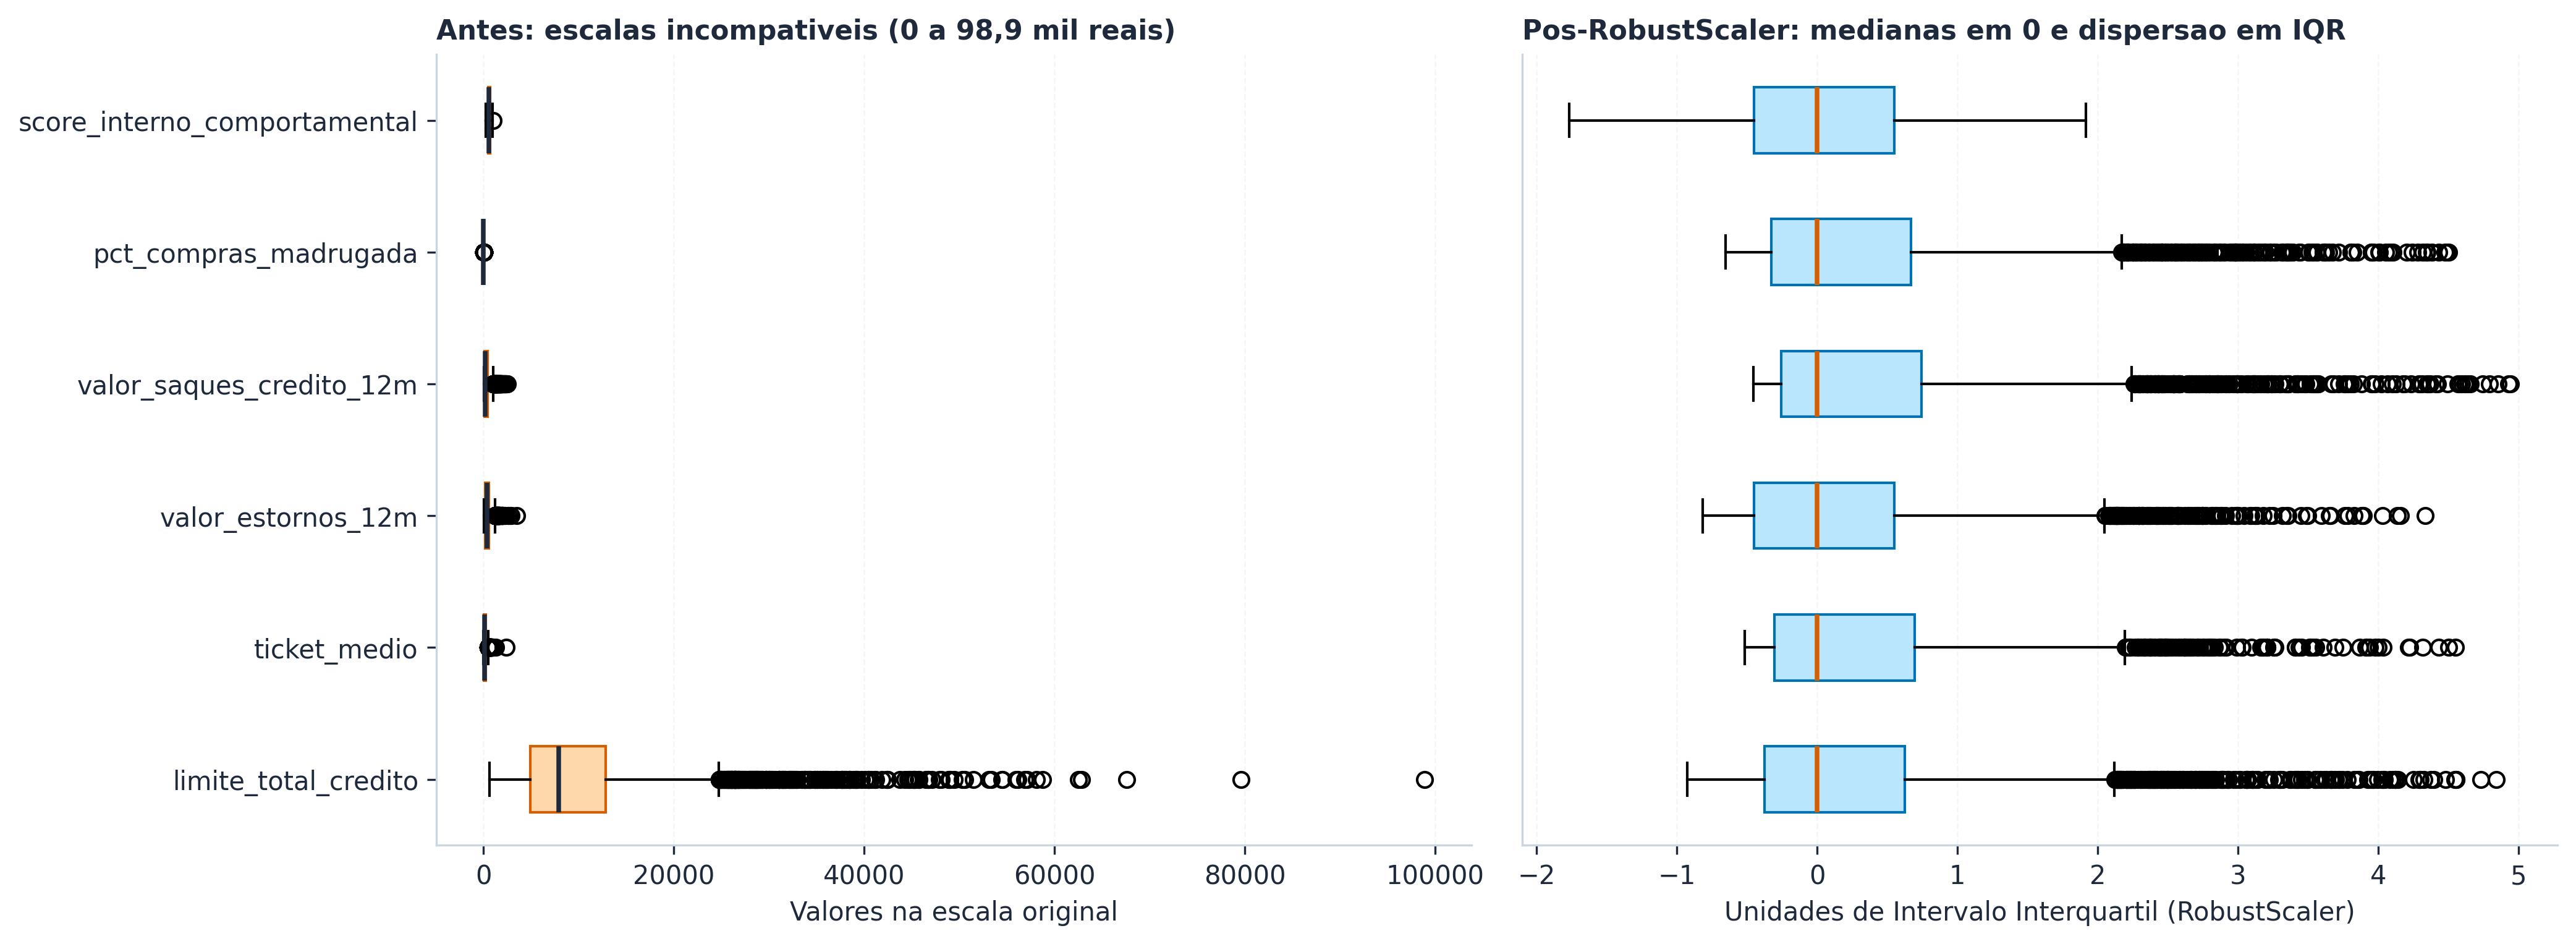
\includegraphics[width=0.98\columnwidth]{../imagens/fig06_comparacao_robust_scaler.png}\\[3pt]
  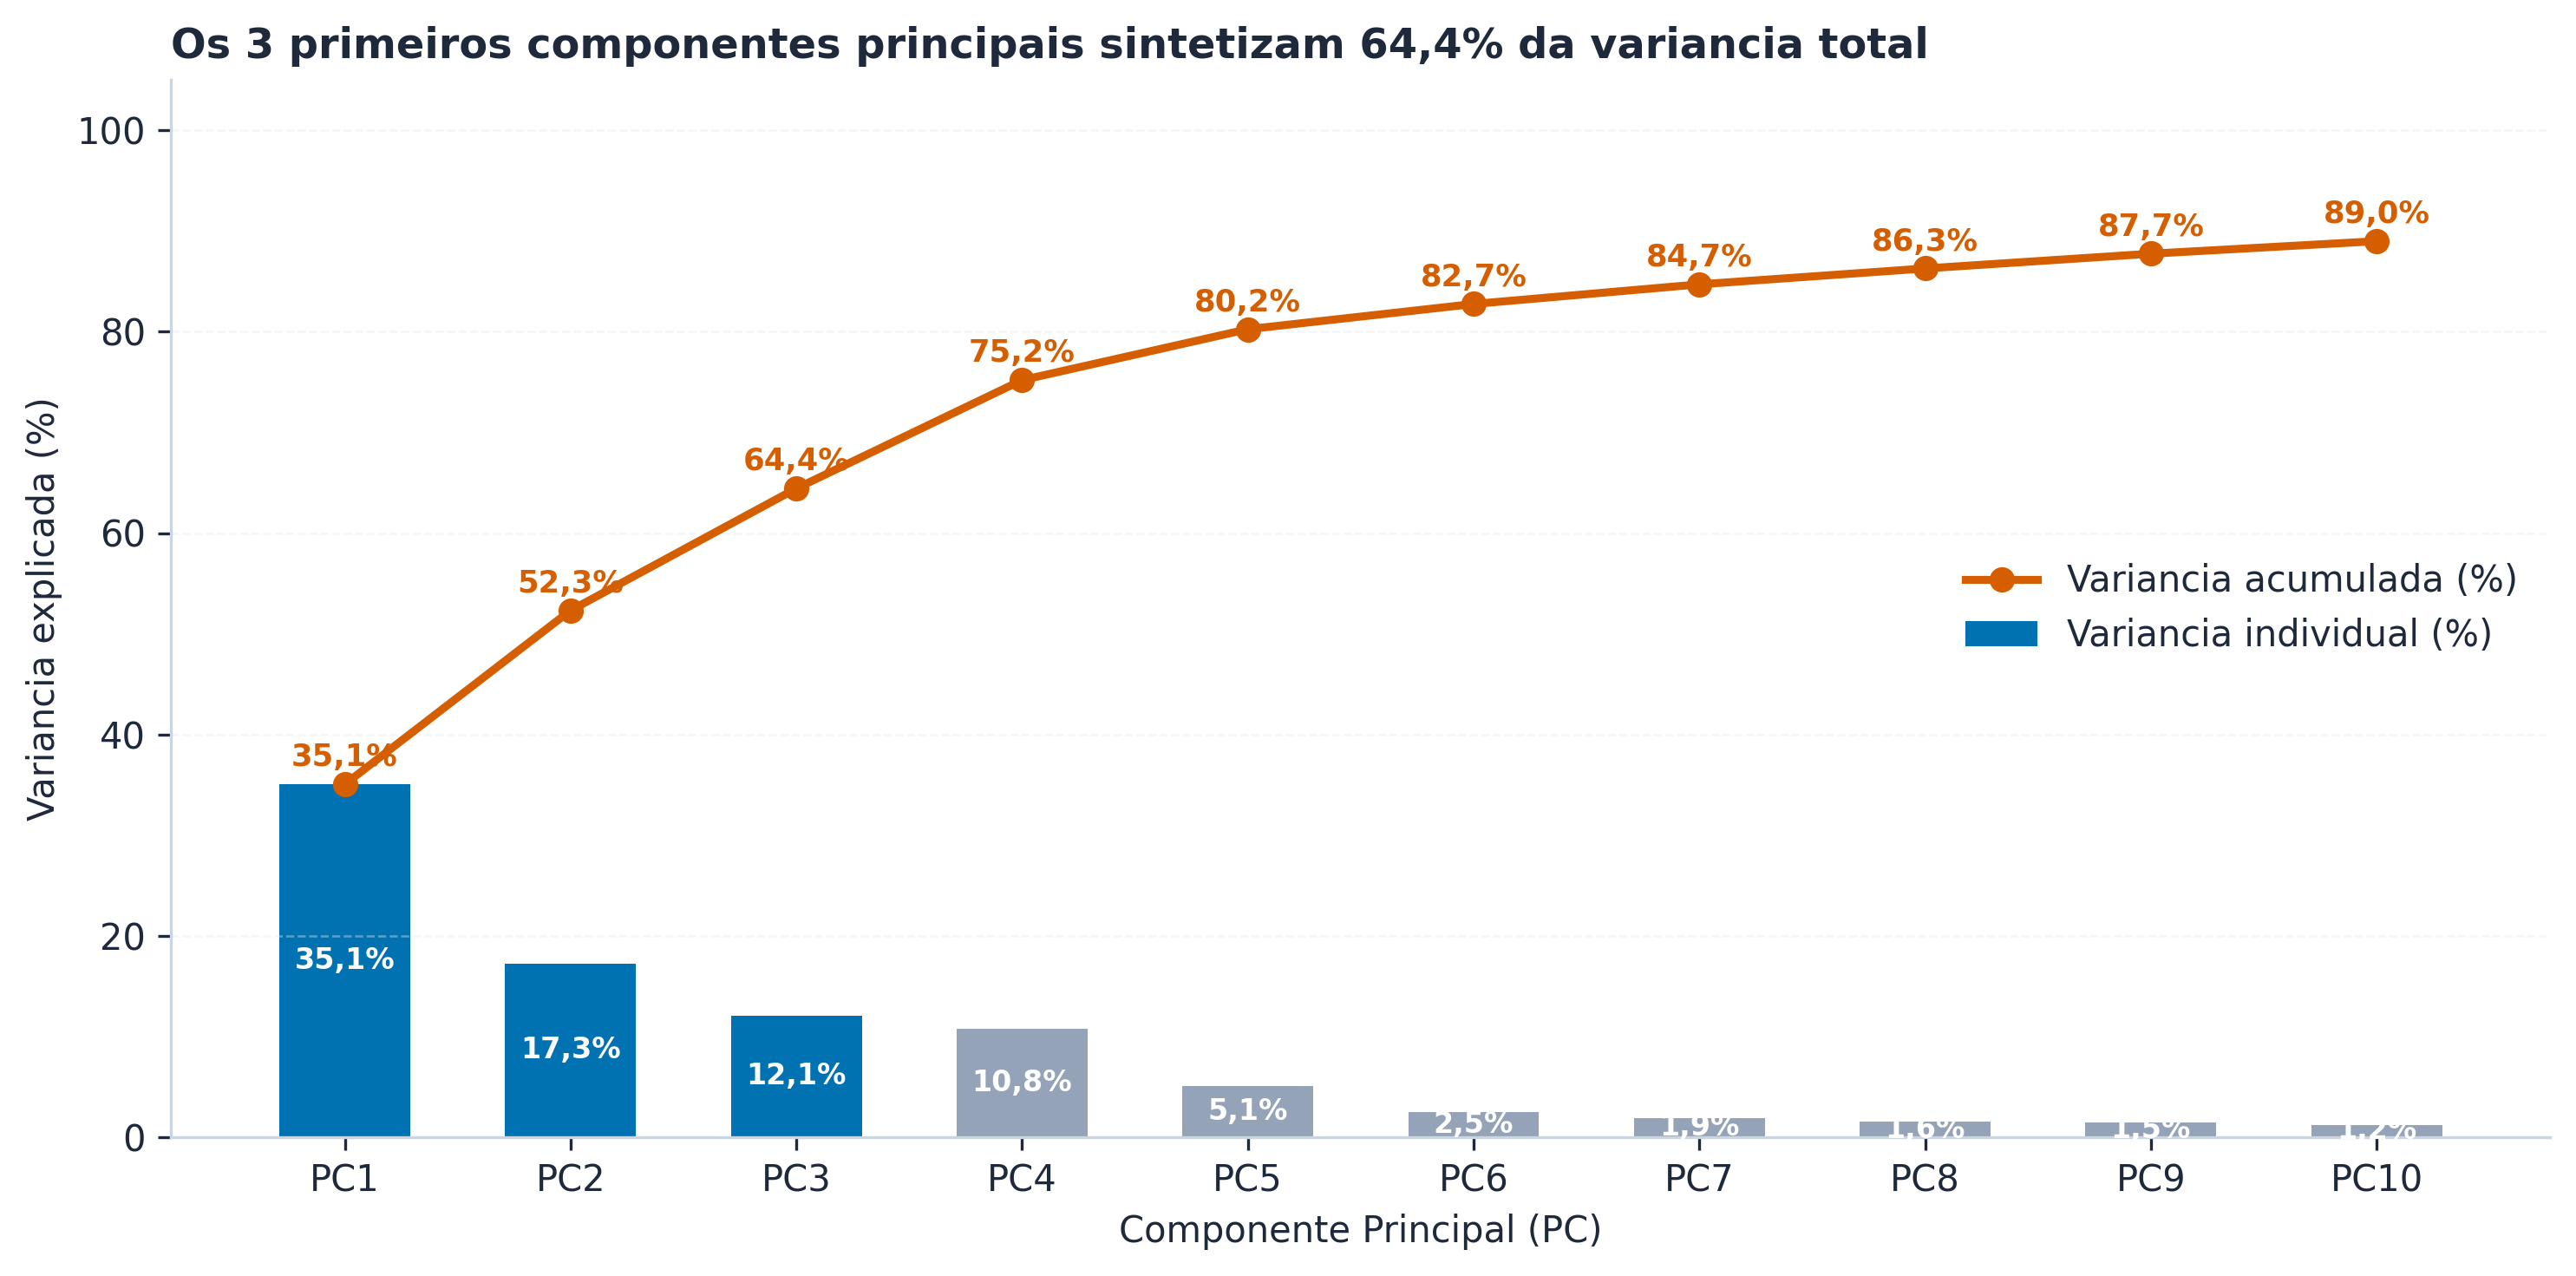
\includegraphics[width=0.98\columnwidth]{../imagens/fig07_pca_variancia_explicada.png}
  \caption{Topo: alinhamento das escalas após \texttt{RobustScaler}. Base: variância explicada individual e acumulada pelos componentes principais (PCA).}
  \label{fig:robust_pca}
\end{figure}

\subsection{Seleção de Atributos e Redução de Dimensionalidade}

A matriz de correlação de Pearson identificou forte multicolinearidade entre variáveis temporais de gasto e volume, como \texttt{gasto\_medio\_mensal\_3m} $\leftrightarrow$ \texttt{gasto\_medio\_mensal\_12m} ($r = 0,9862$), \texttt{qtd\_transacoes\_30d} $\leftrightarrow$ \texttt{qtd\_transacoes\_90d} ($r = 0,9858$) e \texttt{limite\_utilizado\_pct} $\leftrightarrow$ \texttt{gasto\_medio\_mensal\_3m} ($r = 0,9581$). Aplicamos corte em $|r| > 0,90$, eliminando **$8$ variáveis redundantes** (\texttt{gasto\_medio\_mensal\_3m}, \texttt{gasto\_medio\_mensal\_12m}, \texttt{qtd\_transacoes\_90d}, \texttt{taxa\_estorno\_pct}, \texttt{qtd\_atrasos\_12m}, \texttt{pct\_compras\_internacionais}, \texttt{qtd\_dispositivos\_distintos\_90d} e \texttt{pct\_limite\_comprometido\_parcelas}). \textbf{Por que eliminá-las}: manter atributos quase colineares multiplica artificialmente o peso de um único fator latente na distância euclidiana.

Sobre as $38$ colunas resultantes ($26$ numéricas e $12$ binárias), aplicamos o **PCA**, retendo os **$3$ primeiros componentes principais**, que sintetizam **$64,43\%$ da variância global** ($\text{PC1} = 35,05\%$ ligado a saques no crédito, parcelamentos e idade da conta; $\text{PC2} = 17,26\%$ ligado a limite utilizado, compras na madrugada e trocas cadastrais; e $\text{PC3} = 12,11\%$ ligado a pagamento mínimo e frequência em $30$ dias), conforme a Figura~\ref{fig:robust_pca} (base). \textbf{Por que não escolhemos t-SNE ou UMAP}: por serem projeções não lineares estocásticas voltadas apenas à visualização, t-SNE e UMAP deformam densidades locais e distâncias globais, invalidando o cálculo de vizinhança do DBSCAN e a covariância do GMM.

\subsection{Escolha dos Modelos, Baseline e Uso Operacional}

Selecionamos três algoritmos de naturezas distintas e complementares frente ao perfil da Base 04:
\begin{enumerate}
  \item \textbf{Baseline -- K-Means (Particional)}: minimiza a inércia intracluster $\text{WCSS} = \sum_{k=1}^{K}\sum_{\mathbf{x}_i \in S_k}\|\mathbf{x}_i - \boldsymbol{\mu}_k\|^2$ \cite{macqueen1967}. Estabelece a referência de partição rígida via Método do Cotovelo, mas assume grupos esféricos e absorve anomalias nos grupos regulares.
  \item \textbf{Detecção de Fraudes -- DBSCAN (Densidade)}: define clusters como regiões densas com ao menos $\text{min\_samples}$ vizinhos dentro do raio $\varepsilon$ \cite{ester1996}. Observações em regiões esparsas recebem o rótulo $-1$, isolando combinações multivariadas fraudulentas sem forçá-las a um centróide.
  \item \textbf{Segmentação de Clientes -- GMM (Probabilístico)}: modela a carteira como mistura de $K$ gaussianas $p(\mathbf{x}_i) = \sum_{k=1}^{K}\pi_k \mathcal{N}(\mathbf{x}_i \mid \boldsymbol{\mu}_k, \boldsymbol{\Sigma}_k)$ com matriz de covariância completa (\texttt{full}) \cite{dempster1977,reynolds2009}. Permite que um cliente pertença simultaneamente a mais de um grupo com probabilidade a posteriori $\gamma_{ik} = P(c_k \mid \mathbf{x}_i)$, capturando perfis em transição.
\end{enumerate}

\subsection{Métricas de Avaliação e Como Interpretá-las}

Como a base não possui rótulos de fraude, a qualidade dos agrupamentos é validada por métricas internas geométricas, de densidade e probabilísticas:
\begin{itemize}
  \item \textbf{WCSS / Inércia (K-Means)}: mede a distância interna dos clientes ao centro do seu grupo. \textit{Como ler}: valores menores indicam grupos mais compactos; escolhe-se o ponto de ``cotovelo'', onde adicionar novos grupos traz pouco ganho.
  \item \textbf{Coeficiente de Silhouette} ($[-1, +1]$): compara a proximidade do cliente ao seu próprio grupo com a distância ao grupo vizinho \cite{rousseeuw1987}. \textit{Como ler}: **quanto mais próximo de $+1$, melhor** (acima de $0,40$ em dados reais indica boa separação; próximo de $0$ indica sobreposição).
  \item \textbf{Índice de Davies-Bouldin (DB)}: razão entre a dispersão interna e a distância entre clusters. \textit{Como ler}: **quanto menor (mais próximo de $0$), melhor** e menos sobrepostos são os grupos.
  \item \textbf{Índice de Calinski-Harabasz (CH)}: razão entre a variância entre grupos e a variância interna. \textit{Como ler}: **quanto maior o valor, melhor** e mais bem definidos são os clusters.
  \item \textbf{Taxa de Ruído e Razão de Isolamento (DBSCAN)}: medem a fração de anomalias ($\text{cluster} = -1$) e quantas vezes elas estão mais distantes do $15^\circ$ vizinho do que um cliente normal. \textit{Como ler}: uma taxa de ruído entre $1\%$ e $5\%$ com razão de isolamento $> 2\times$ confirma que as suspeitas de fraude estão de fato isoladas em regiões esparsas.
  \item \textbf{BIC, AIC e Certeza a Posteriori (GMM)}: o BIC e o AIC medem o ajuste probabilístico penalizando o excesso de parâmetros, enquanto $\overline{P_{\max}}$ mede a probabilidade média do grupo vencedor. \textit{Como ler}: **quanto menor o BIC/AIC, melhor** é o número de grupos sem sobreajuste; clientes com $P_{\max} < 0,80$ indicam perfis híbridos na fronteira entre dois hábitos de consumo.
\end{itemize}

\section{Resultados e Discussão}

A Figura~\ref{fig:hyperparams} consolida a seleção de hiperparâmetros dos três modelos no espaço PCA. No \textit{baseline} K-Means, a curva WCSS apresenta cotovelo em **$k = 4$** ($14,96$ mil) e o índice de Calinski-Harabasz atinge seu máximo global ($4.244,4$), com Silhouette de $0,4183$. No GMM, o Critério de Informação Bayesiano (BIC) decresce até atingir seu ponto mínimo exatamente em **$k = 4$ ($49.963,7$)**, voltando a subir em $k = 5$ ($49.988,6$). No DBSCAN, a curva \textit{k-distance} para $k = 15$ vizinhos identifica o joelho de inflexão da cauda em **$\varepsilon = 0,75$**, isolando **$232$ clientes ($5,00\%$ da base limpa) como anomalias espaciais ($\text{cluster} = -1$)**.

\begin{figure}[htbp]
  \centering
  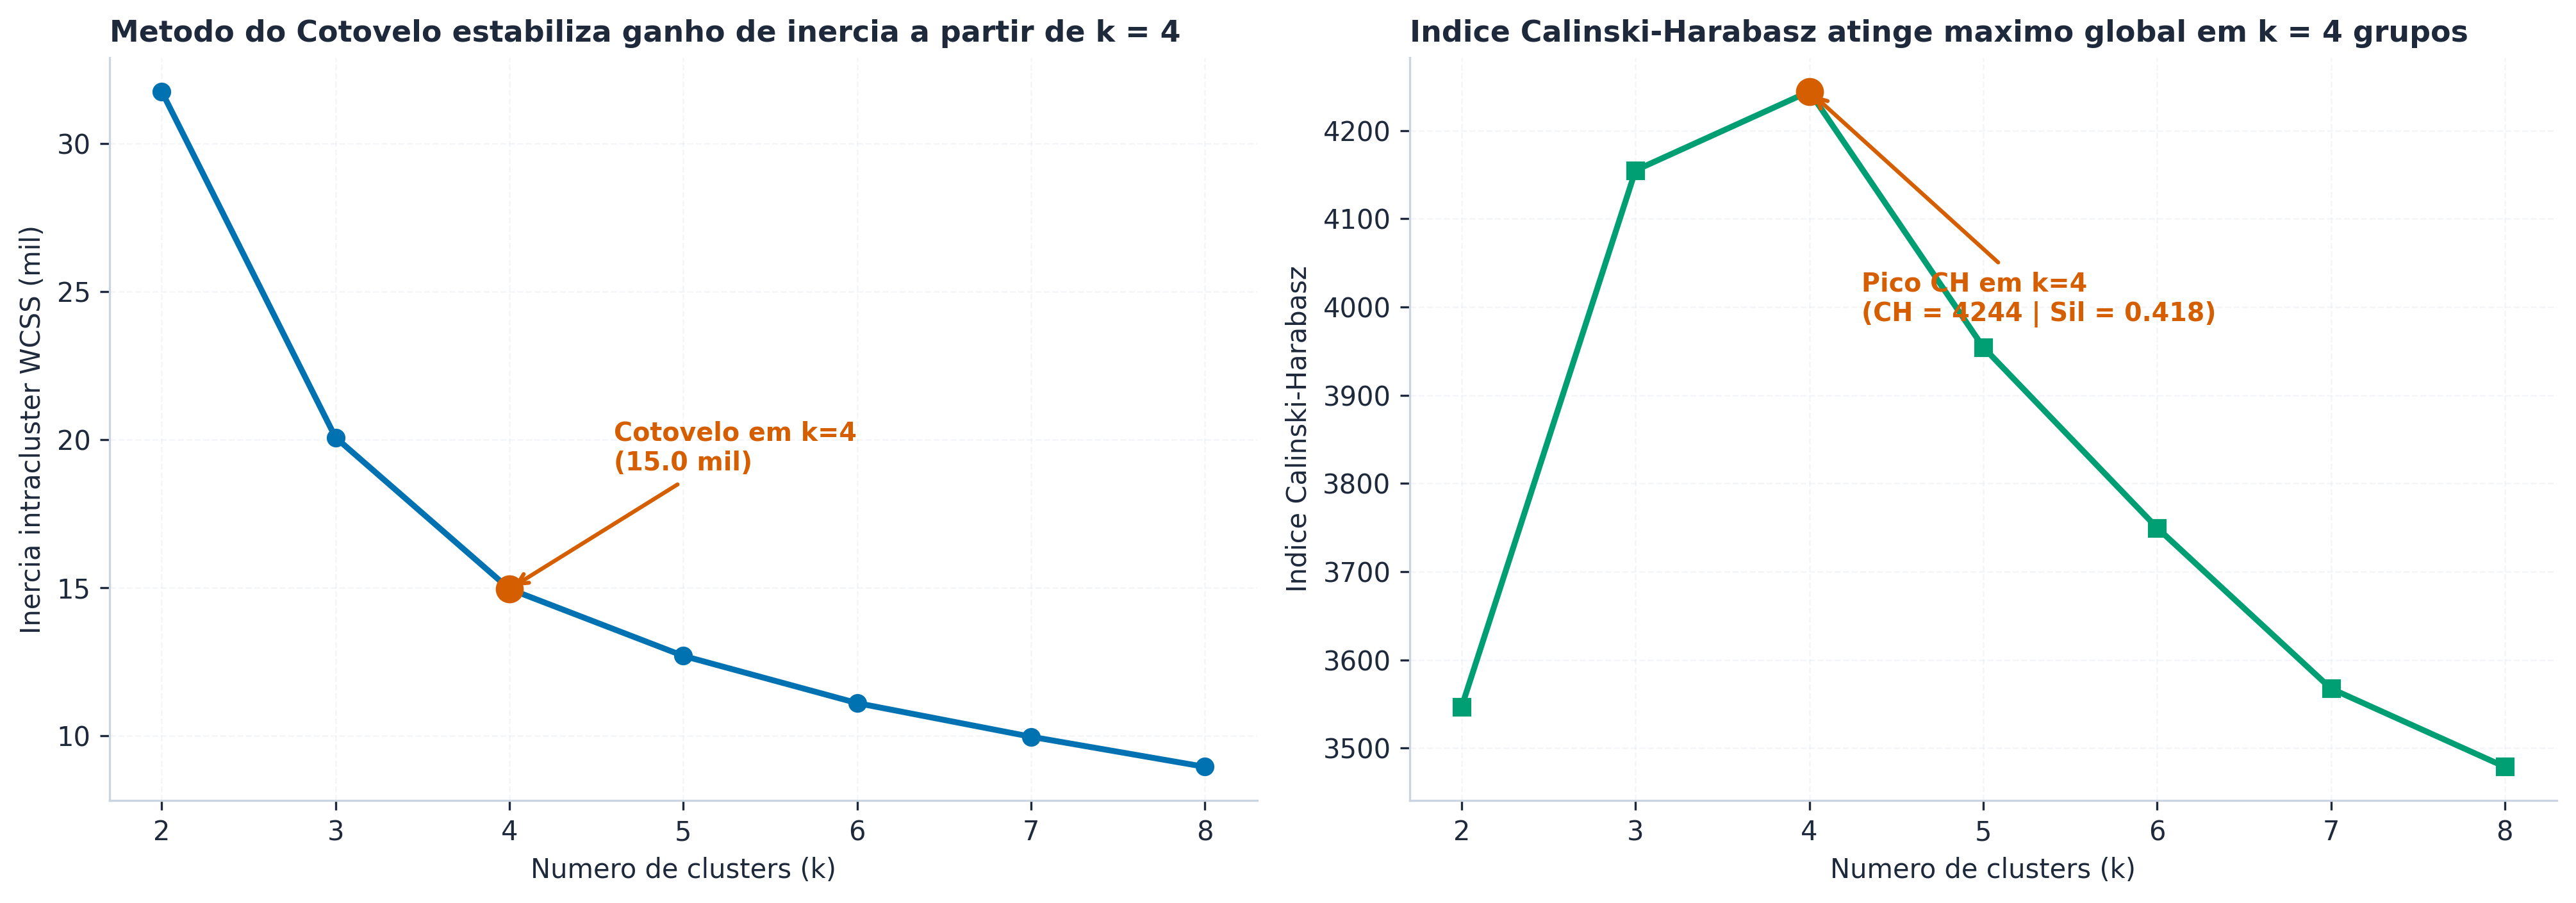
\includegraphics[width=0.98\columnwidth]{../imagens/fig08_kmeans_cotovelo.png}\\[3pt]
  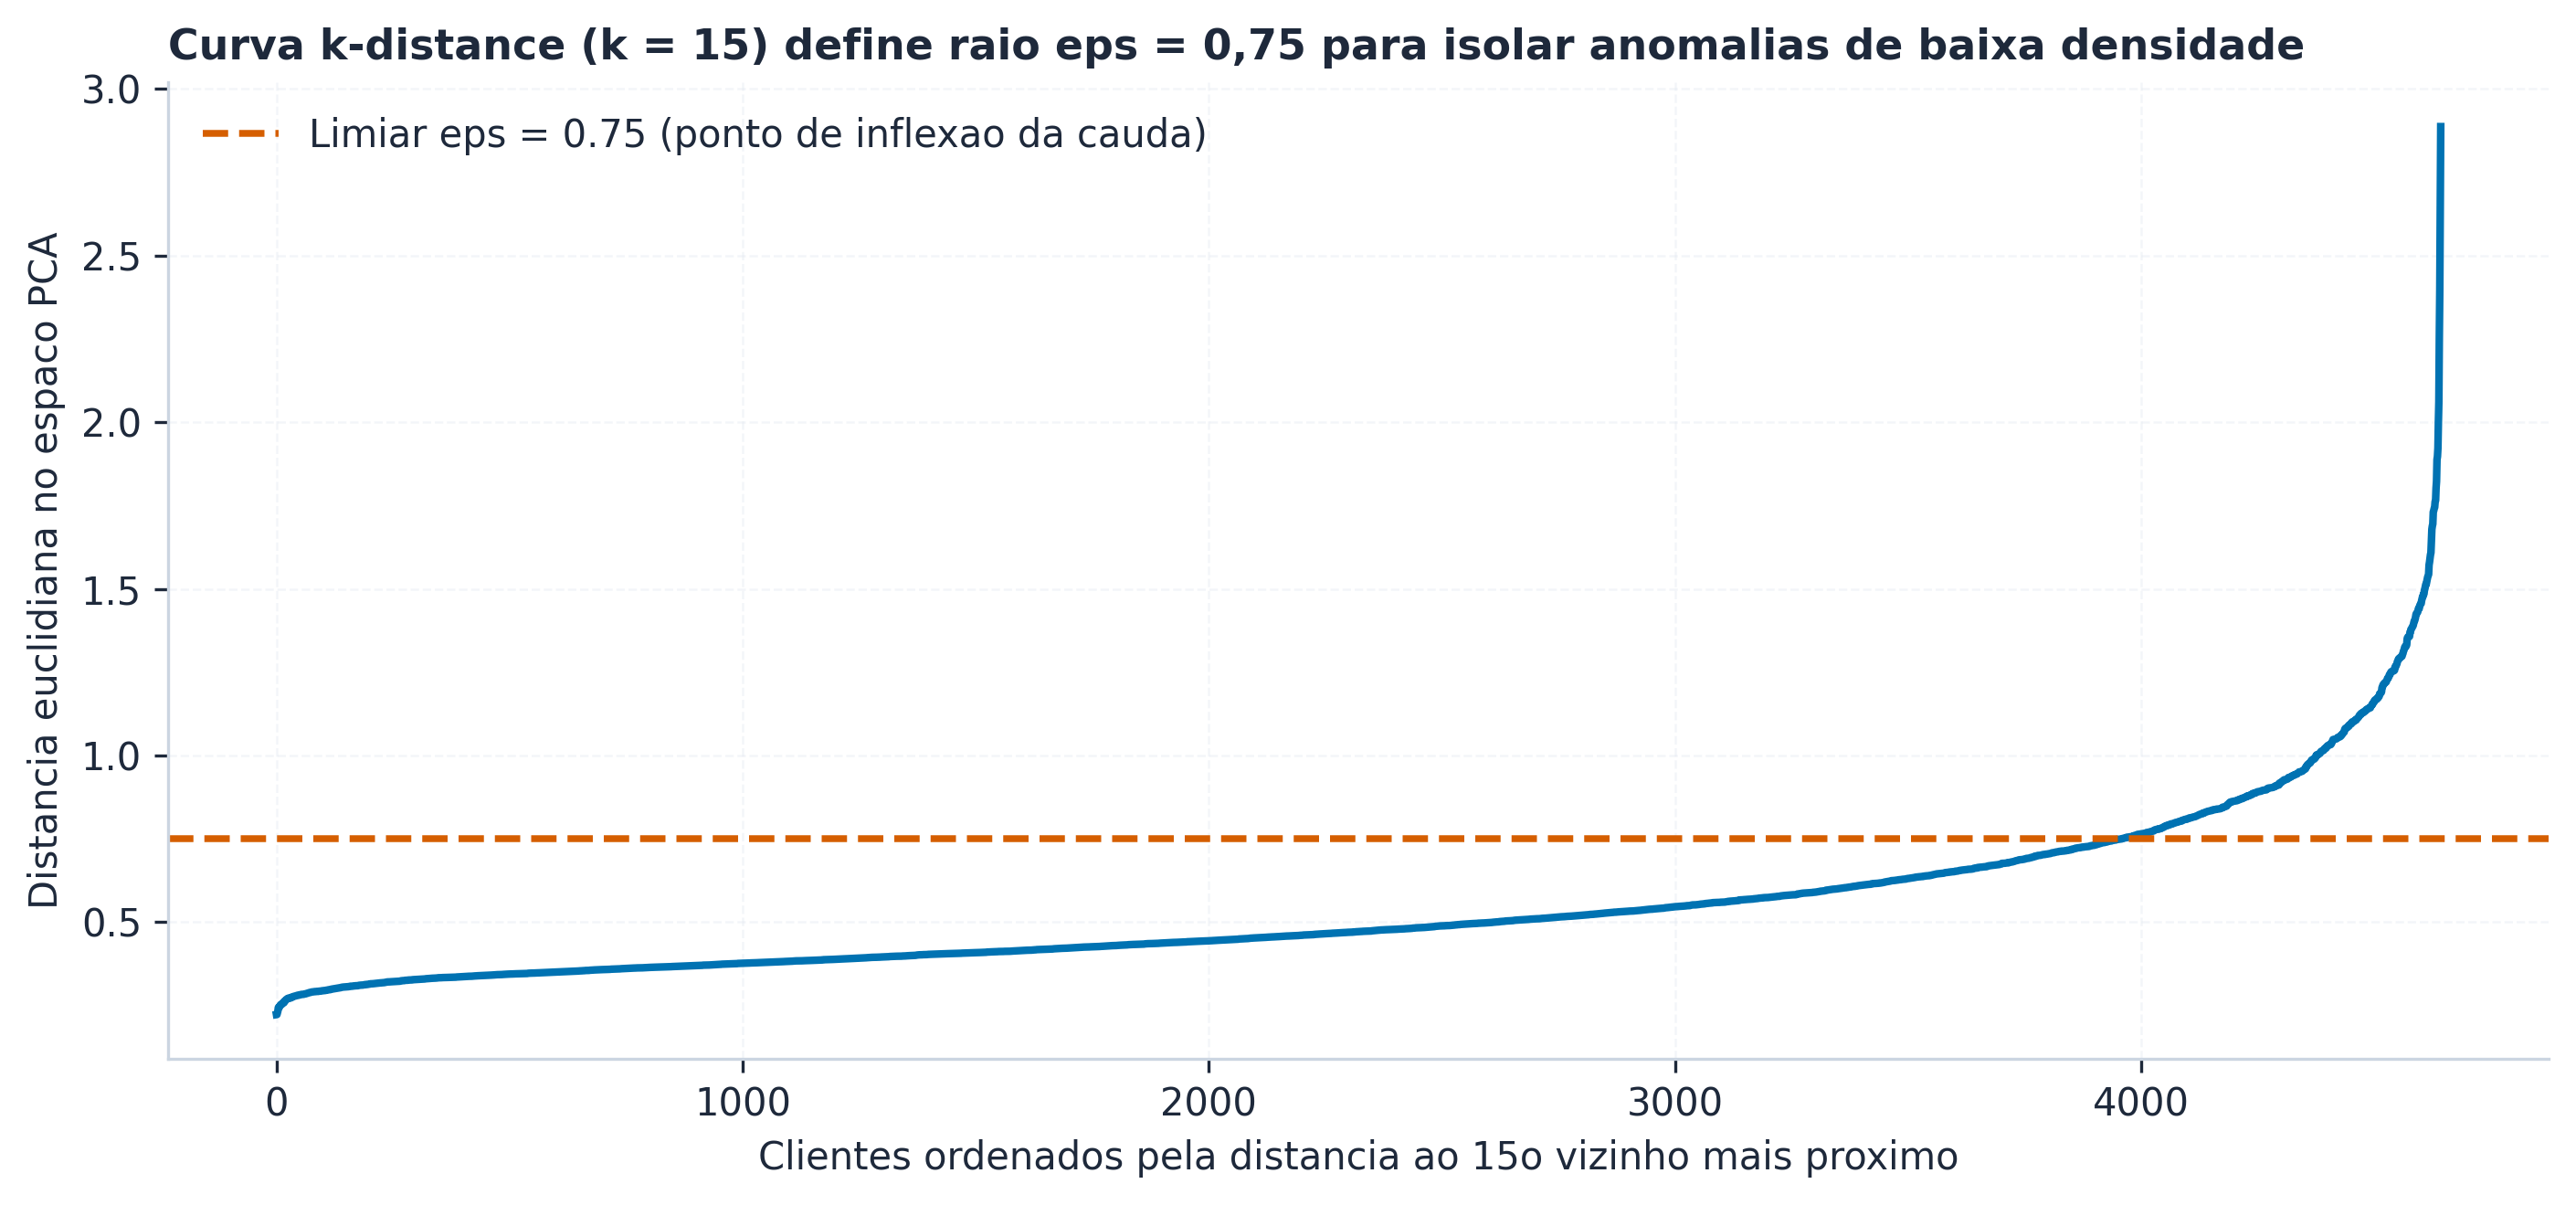
\includegraphics[width=0.48\columnwidth]{../imagens/fig09_dbscan_kdistance.png}\hfill
  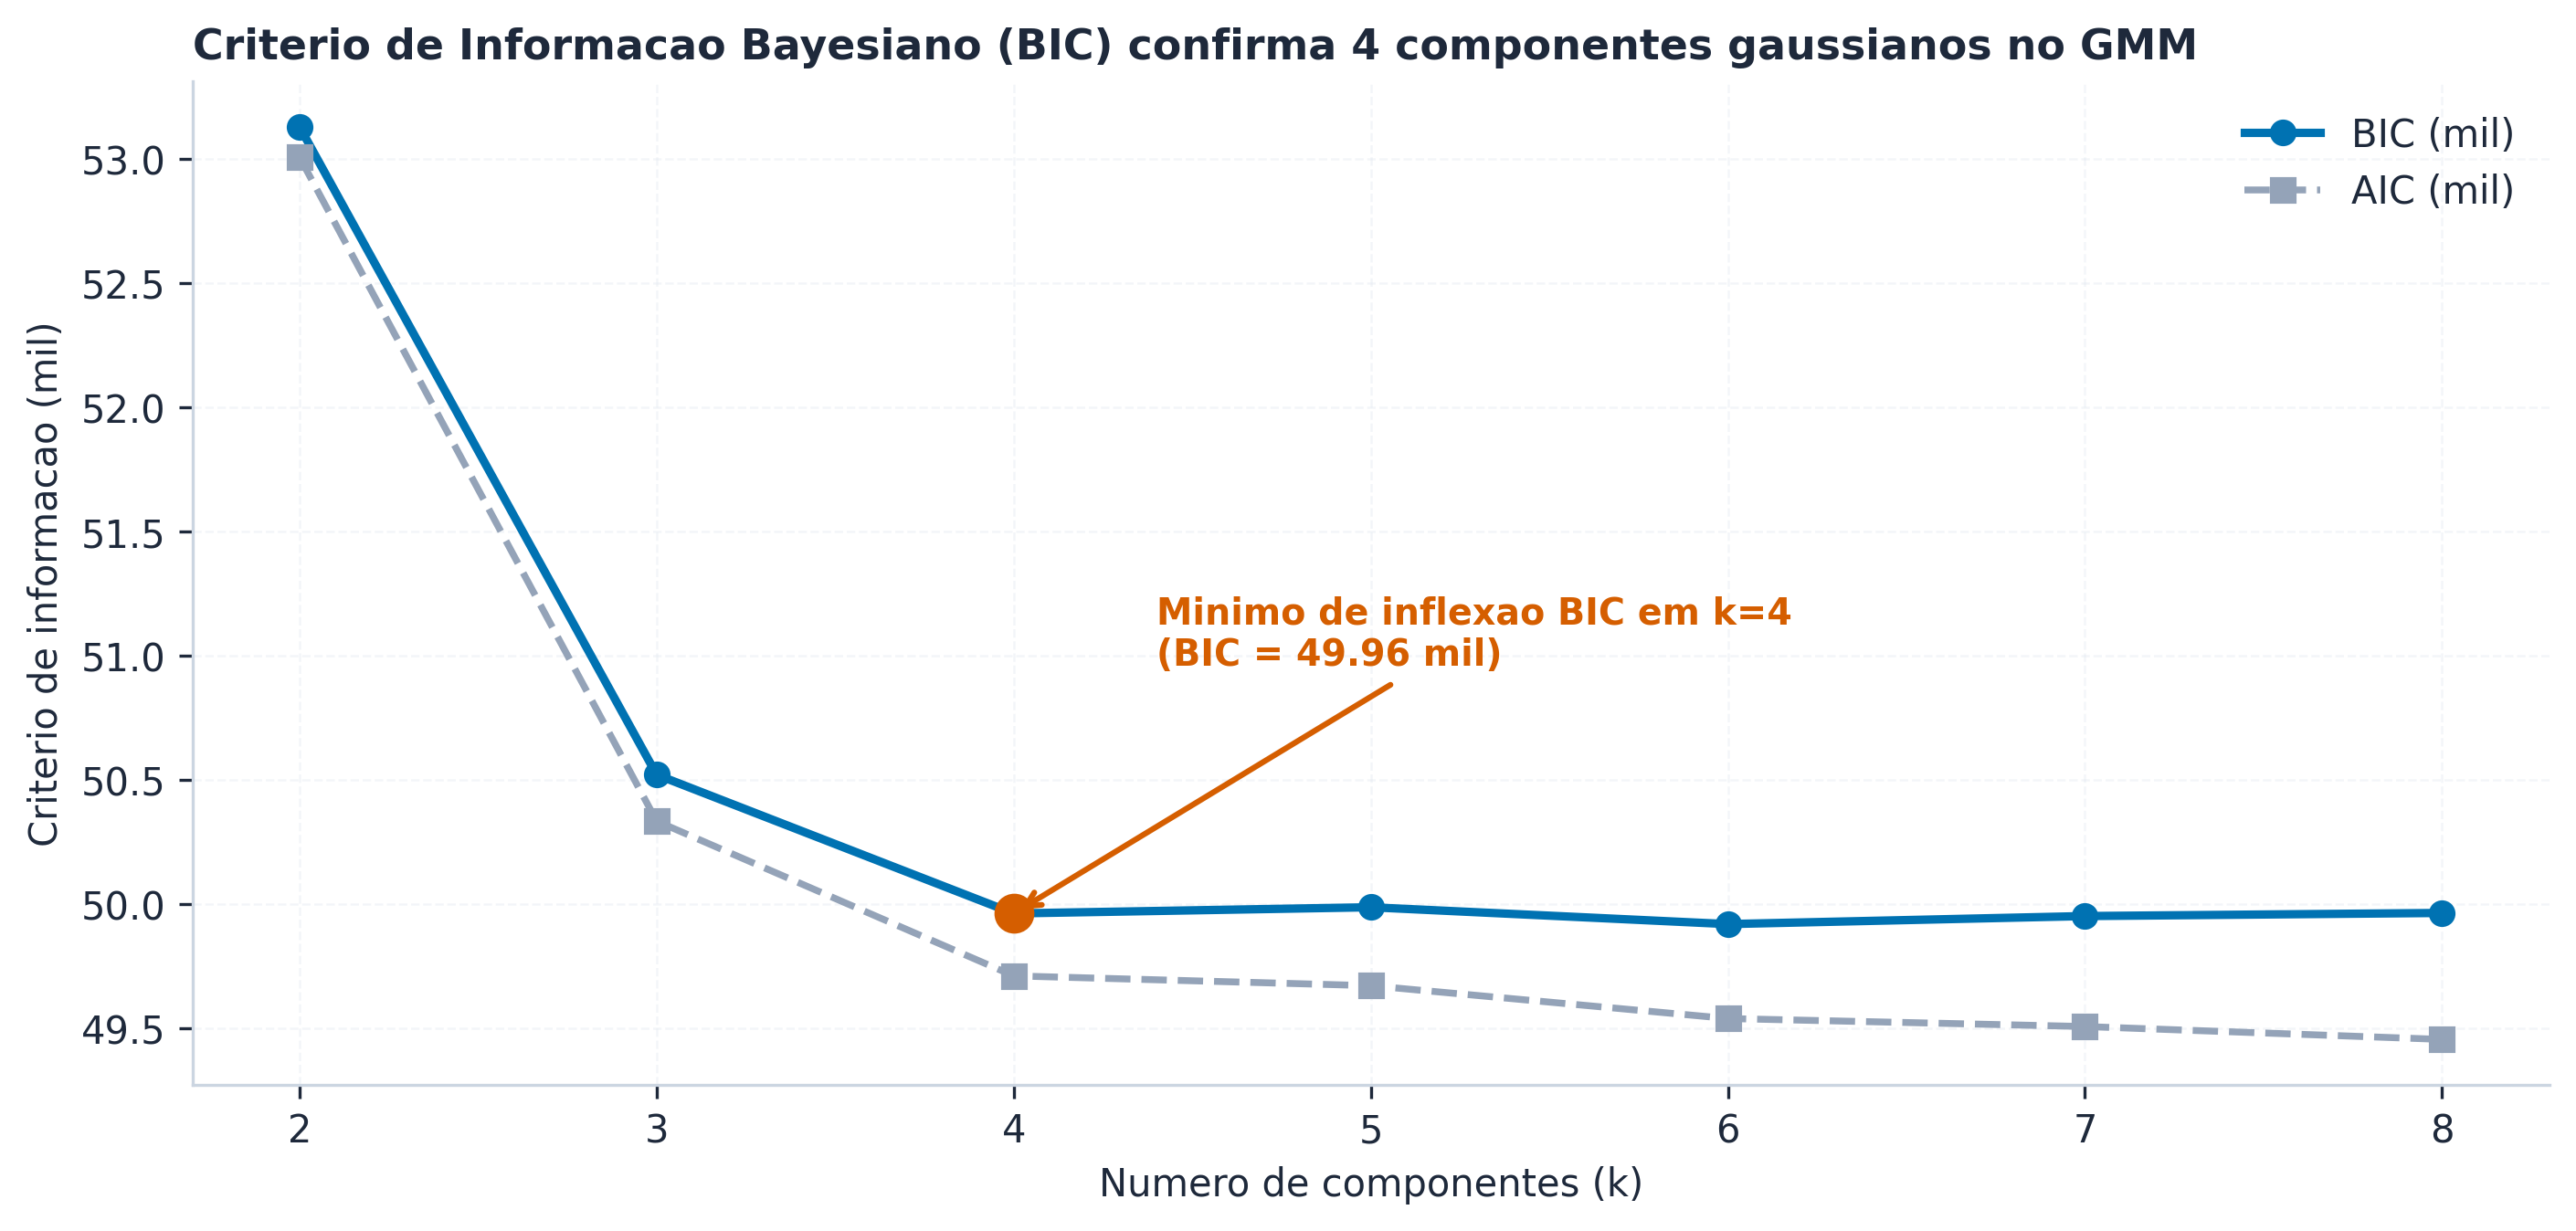
\includegraphics[width=0.48\columnwidth]{../imagens/fig10_gmm_bic_aic.png}
  \caption{Topo: Método do Cotovelo e Calinski-Harabasz no K-Means ($k=4$). Base esq.: curva \textit{k-distance} do DBSCAN ($\varepsilon=0,75$). Base dir.: seleção de $k=4$ pelo BIC no GMM.}
  \label{fig:hyperparams}
\end{figure}

A Tabela~\ref{tab:metrics_comp} resume as métricas de validação dos três modelos:
\begin{itemize}
  \item \textbf{Métricas Específicas do DBSCAN}: Além das métricas geométricas sobre os núcleos densos (Silhouette $= 0,4462$, Davies-Bouldin $= 0,7746$ e Calinski-Harabasz $= 3.694,5$, frente ao Silhouette global com ruído de $0,3621$), avaliamos a **Taxa de Ruído** ($5,00\%$, $232$ anomalias), a **Proporção de \textit{Core Points}** ($84,65\%$, $3.931$ pontos centrais e $481$ pontos de borda) e a **Razão de Isolamento Espacial** ($d_{15}(\text{anomalia}) / d_{15}(\text{normal}) = 2,21\times$, pois a distância média ao $15^\circ$ vizinho salta de $0,4672$ nos clientes normais para $1,0328$ nas anomalias).
  \item \textbf{Métricas Específicas do GMM ($k = 4$)}: Além de Silhouette ($0,4095$), Davies-Bouldin ($0,8992$) e Calinski-Harabasz ($4.088,1$), o ajuste probabilístico é validado pelo **BIC** ($49.963,7$), **AIC** ($49.712,4$), **Log-Verossimilhança Média** ($-5,3375$ por amostra), **Entropia Média de Shannon** ($H = 0,1042$, indicando baixa incerteza global), **Certeza Média a Posteriori** ($\overline{P_{\max}} = 95,46\%$) e **Taxa de Clientes em Transição** ($4,16\%$, $193$ clientes com $P_{\max} < 0,80$).
\end{itemize}

\begin{table}[htbp]
  \centering
  \caption{Métricas de validação interna e detecção de ruídos/transições no espaço PCA (3D).}
  \label{tab:metrics_comp}
  \resizebox{\columnwidth}{!}{%
  \begin{tabular}{lccccc}
    \toprule
    \textbf{Modelo} & \textbf{Grupos} & \textbf{Silhouette} & \textbf{Davies-Bouldin} & \textbf{Calinski-Harabasz} & \textbf{Anomalias / Transição} \\
    \midrule
    K-Means (\textit{Baseline}) & $4$ & $0,4183$ & $0,8796$ & $4.244,4$ & $0$ (partição rígida) \\
    DBSCAN ($\varepsilon=0,75, ms=15$) & $2$ (+ruído) & $0,4462^*$ & $0,7746^*$ & $3.694,5^*$ & $232$ ruídos ($5,00\%$) \\
    GMM ($k=4$, \textit{full cov.}) & $4$ & $0,4095$ & $0,8992$ & $4.088,1$ & $193$ híbridos ($P_{\max}<0,80$) \\
    \bottomrule
  \end{tabular}%
  }
  \footnotesize{\\ $^*$Métricas do DBSCAN avaliadas sobre os pontos pertencentes aos núcleos densos ($\text{cluster} \neq -1$).}
\end{table}

\begin{figure*}[htbp]
  \centering
  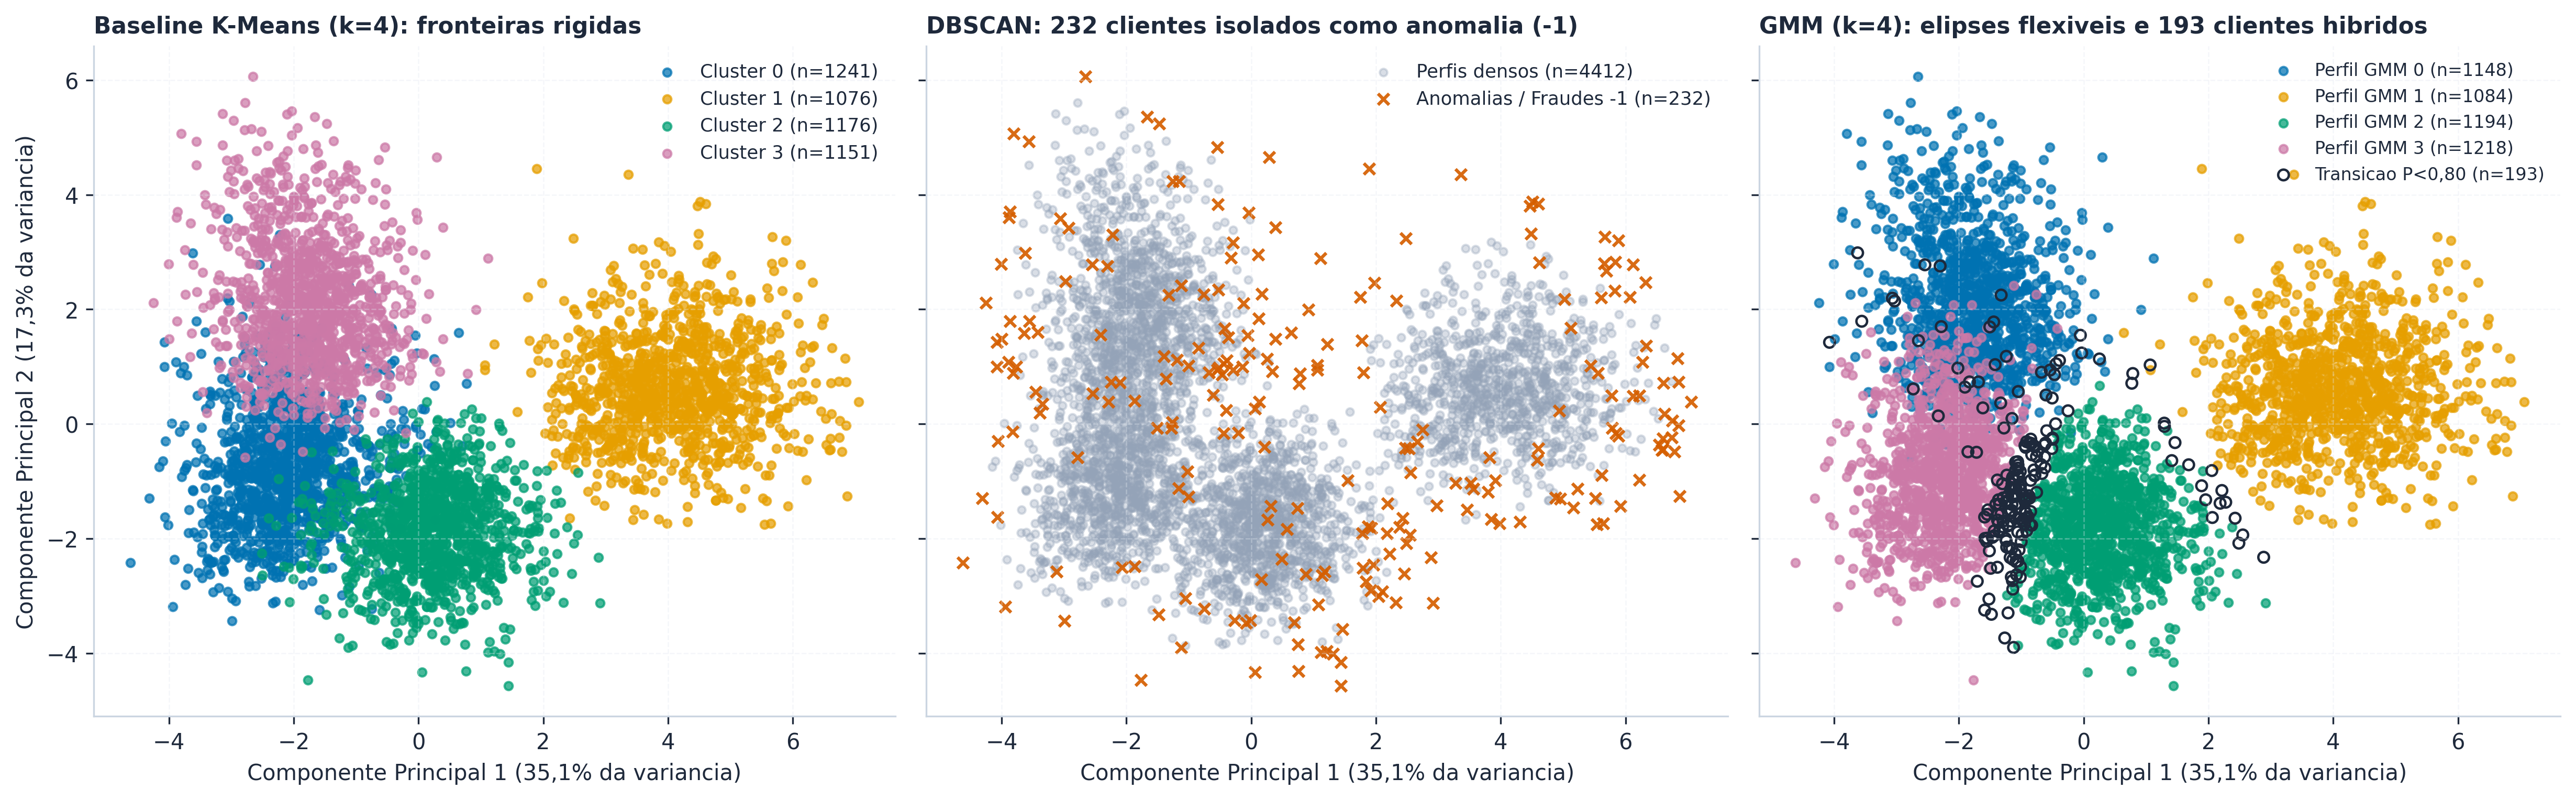
\includegraphics[width=0.96\textwidth]{../imagens/fig11_comparacao_clusters_pca2d.png}
  \caption{Projeção no plano $\text{PC1} \times \text{PC2}$ ($52,3\%$ da variância): (a) partição rígida do K-Means; (b) isolamento das 232 anomalias periféricas ($\text{cluster} = -1$) pelo DBSCAN; e (c) elipses do GMM com os 193 clientes em transição probabilística ($P_{\max} < 0,80$).}
  \label{fig:pca_2d_comp}
\end{figure*}

A projeção 2D no espaço PCA (Figura~\ref{fig:pca_2d_comp}) e o cruzamento das variáveis originais na Tabela~\ref{tab:profiles} revelam a estrutura operacional dos quatro segmentos do GMM e das anomalias do DBSCAN:
\begin{itemize}
  \item \textbf{G0 -- Alto Consumo Internacional ($n = 1.148$, $24,7\%$)}: Maior gasto mensal (R\$ $6.977,32$), maior ticket médio (R\$ $293,67$), alta utilização do limite ($66,94\%$) e $22,24\%$ de compras internacionais, sem contestações ($0,00$) nem atrasos ($0,05$), mas com uso relevante de pagamento mínimo ($22,50\%$).
  \item \textbf{G1 -- Veteranos Digitais e Saques ($n = 1.084$, $23,3\%$)}: Contas mais antigas ($79,34$ meses), maior limite (R\$ $14.762,08$), maior score ($762,52$) e $86,95\%$ de pagamento total. Concentram $73,31\%$ das compras online com ticket baixo (R\$ $45,17$), mas lideram em saques no crédito (R\$ $727,23$/ano), taxa de estorno ($7,81\%$) e contestações ($1,22$/ano), indicando exposição a clonagem digital em e-commerce.
  \item \textbf{G2 -- Varejo com Instabilidade Cadastral ($n = 1.194$, $25,7\%$)}: Menor limite (R\$ $6.879,22$) e compras frequentes ($34,30$/mês), porém registra a **maior média de alterações cadastrais ($3,19$/ano)** combinada a contestações ($1,21$/ano) e compras na madrugada ($8,42\%$), assinatura clássica de tomada de conta (\textit{Account Takeover}).
  \item \textbf{G3 -- Jovens Noturnos e Rotativo ($n = 1.218$, $26,2\%$)}: Contas recentes ($20,52$ meses), menor pagamento integral ($43,38\%$) e **maior proporção de compras na madrugada ($13,82\%$)** com $2,42$ alterações cadastrais/ano.
  \item \textbf{Anomalias DBSCAN ($-1$, $n = 232$, $5,0\%$)**: Espalhadas transversalmente pelos quatro grupos ($55$ do G0, $86$ do G1, $53$ do G2 e $38$ do G3), combinam a maior velocidade transacional ($42,22$ compras/30d), o maior uso de pagamento mínimo ($26,38\%$), limites elevados (R\$ $12.605,78$) e alto volume simultâneo de saques no crédito (R\$ $536,24$) e estornos (R\$ $446,17$).
\end{itemize}

\begin{table*}[htbp]
  \centering
  \caption{Perfil médio das variáveis originais nos quatro segmentos do GMM e no lote de anomalias isolado pelo DBSCAN ($-1$).}
  \label{tab:profiles}
  \resizebox{0.96\textwidth}{!}{%
  \begin{tabular}{lccccc}
    \toprule
    \textbf{Variável Original (Média)} & \textbf{G0: Alto Consumo Int.} & \textbf{G1: Veteranos Digitais} & \textbf{G2: Varejo / Troca Cad.} & \textbf{G3: Jovens Noturnos} & \textbf{DBSCAN (-1): Anomalias} \\
    \midrule
    Clientes ($n$ / $\%$) & $1.148$ ($24,7\%$) & $1.084$ ($23,3\%$) & $1.194$ ($25,7\%$) & $1.218$ ($26,2\%$) & $232$ ($5,0\%$ transversal) \\
    Limite total (R\$) / Uso ($\%$) & $8.967,90$ / $\mathbf{66,94\%}$ & $\mathbf{14.762,08}$ / $21,05\%$ & $6.879,22$ / $20,68\%$ & $8.608,66$ / $37,73\%$ & $12.605,78$ / $33,69\%$ \\
    Gasto 3m (R\$) / Ticket médio (R\$) & $\mathbf{6.977,32}$ / $\mathbf{293,67}$ & $1.248,71$ / $45,17$ & $1.660,81$ / $57,32$ & $2.961,92$ / $196,33$ & $3.035,25$ / $147,23$ \\
    Transações 30d ($n$) / Idade (meses) & $28,24$ / $47,07$ & $32,93$ / $\mathbf{79,34}$ & $34,30$ / $41,48$ & $17,72$ / $20,52$ & $\mathbf{42,22}$ / $66,68$ \\
    Pag. total ($\%$) / Pag. mínimo ($\%$) & $59,00\%$ / $22,50\%$ & $\mathbf{86,95\%}$ / $14,60\%$ & $56,72\%$ / $18,17\%$ & $43,38\%$ / $7,20\%$ & $65,51\%$ / $\mathbf{26,38\%}$ \\
    Compras online / Internacionais ($\%$) & $46,39\%$ / $\mathbf{22,24\%}$ & $\mathbf{73,31\%}$ / $2,63\%$ & $32,63\%$ / $3,30\%$ & $27,11\%$ / $6,82\%$ & $48,75\%$ / $8,43\%$ \\
    Compras madrugada ($\%$) / Trocas cad. ($n$) & $4,23\%$ / $0,86$ & $2,56\%$ / $1,27$ & $8,42\%$ / $\mathbf{3,19}$ & $\mathbf{13,82\%}$ / $2,42$ & $6,29\%$ / $1,90$ \\
    Contestações ($n$) / Taxa estorno ($\%$) & $0,00$ / $1,21\%$ & $\mathbf{1,22}$ / $\mathbf{7,81\%}$ & $1,21$ / $4,24\%$ & $0,13$ / $2,32\%$ & $1,05$ / $4,49\%$ \\
    Saques crédito 12m (R\$) / Score interno & $114,59$ / $471,77$ & $\mathbf{727,23}$ / $\mathbf{762,52}$ & $346,55$ / $618,02$ & $84,92$ / $541,18$ & $536,24$ / $619,65$ \\
    \bottomrule
  \end{tabular}%
  }
\end{table*}

\section{Conclusão}

A aplicação da metodologia KDD à Base 04 comprovou que a eliminação de colinearidade ($|r| > 0,90$), o filtro de extremos ($4,0 \times \text{IQR}$), o escalonamento com \texttt{RobustScaler} e a redução via PCA são essenciais para viabilizar o agrupamento em alta dimensão. A atuação conjunta do **DBSCAN** e do **GMM** supera o \textit{baseline} K-Means ao separar a detecção de anomalias da segmentação elíptica probabilística.

Traduzimos os achados técnicos em **quatro ações práticas contra fraudes** para a operadora:
\begin{enumerate}
  \item \textbf{Auditoria e Step-Up Authentication (Anomalias DBSCAN $-1$ e Extremos)}: Exigir biometria facial e \textit{3D-Secure 2.0} para os $232$ clientes isolados pelo DBSCAN e os $356$ outliers extremos sempre que a frequência superar $40$ transações/30d combinada a saques no crédito acima de R\$ $500$.
  \item \textbf{Quarentena Pós-Alteração Cadastral (Grupos 2 e 3)}: Implantar trava preventiva de $24$ horas após alteração de telefone, endereço ou dispositivo nos clientes do G2 ($3,19$ trocas/ano) e G3 ($13,82\%$ de compras na madrugada), bloqueando transações entre $00\text{h}$ e $06\text{h}$ sem validação por token para mitigar \textit{Account Takeover}.
  \item \textbf{Cartão Virtual com CVV Dinâmico (Grupo 1)}: Incentivar o uso obrigatório de cartão virtual temporário para o G1 ($73,31\%$ de compras online e $7,81\%$ de taxa de estorno), protegendo clientes antigos e de alto limite (R\$ $14,76$ mil) contra vazamentos em e-commerce sem reduzir sua aprovação.
  \item \textbf{Política de Limite Orientada por Probabilidades do GMM (Grupo 0 e Híbridos)}: Para os $193$ clientes em zona de transição ($P_{\max} < 0,80$), automatizar a concessão de limite apenas quando a probabilidade mensal $P(\text{G0}) + P(\text{G1})$ superar $80\%$, bloqueando aumentos para contas que migrarem em direção ao G2 ou G3.
\end{enumerate}

{\footnotesize
\begin{thebibliography}{9}
\setlength{\itemsep}{1pt}

\bibitem{dempster1977}
Dempster, A.~P., Laird, N.~M., and Rubin, D.~B. (1977).
\newblock Maximum likelihood from incomplete data via the {EM} algorithm.
\newblock {\em Journal of the Royal Statistical Society: Series B}, 39(1):1--22.

\bibitem{ester1996}
Ester, M., Kriegel, H.-P., Sander, J., and Xu, X. (1996).
\newblock A density-based algorithm for discovering clusters in large spatial databases with noise.
\newblock In {\em Proc. of KDD-96}, pages 226--231. AAAI Press.

\bibitem{esteves2025}
Esteves, L.~M. and Gioia, H.~R. (2025).
\newblock Segmentação de clientes financeiros por clusterização e aprendizado não supervisionado (Segmentação estatística de clientes bancários por padrões comportamentais).
\newblock {\em Revista E\&S}. Disponível em: \url{https://revistaes.com.br/resumo-executivo/segmentacao-estatistica-de-clientes-bancarios-por-padroes-comportamentais}.

\bibitem{fayyad1996}
Fayyad, U., Piatetsky-Shapiro, G., and Smyth, P. (1996).
\newblock From data mining to knowledge discovery in databases.
\newblock {\em AI Magazine}, 17(3):37--54.

\bibitem{jolliffe2002}
Jolliffe, I.~T. (2002).
\newblock {\em Principal Component Analysis}.
\newblock Springer, New York, 2nd edition.

\bibitem{macqueen1967}
MacQueen, J. (1967).
\newblock Some methods for classification and analysis of multivariate observations.
\newblock In {\em Proc. 5th Berkeley Symp. on Math. Statistics and Probability}, volume~1, pages 281--297.

\bibitem{reynolds2009}
Reynolds, D.~A. (2009).
\newblock Gaussian mixture models.
\newblock {\em Encyclopedia of Biometrics}, pages 659--663. Springer.

\bibitem{rousseeuw1987}
Rousseeuw, P.~J. (1987).
\newblock Silhouettes: A graphical aid to the interpretation and validation of cluster analysis.
\newblock {\em J. Comput. Appl. Math.}, 20:53--65.

\bibitem{santos2023}
Santos, R.~P.~d. (2023).
\newblock Segmentação comportamental de clientes usando agrupamento automático de dados.
\newblock TCC, ICT-UNIFESP, São José dos Campos. Disponível em: \url{https://repositorio.unifesp.br/items/7efdd05c-afa7-4111-aaa9-b62e1fba4e0b}.

\end{thebibliography}
}

\end{document}
